\documentclass[conference, letterpaper, 11pt]{IEEEtran}

\IEEEoverridecommandlockouts
% The preceding line is only needed to identify funding in the first footnote. If that is unneeded, please comment it out.

\usepackage[style=ieee]{biblatex}
\usepackage{hyperref}
\usepackage{amsmath,amssymb,amsfonts}
\usepackage{algorithmic}
\usepackage{graphicx}
\usepackage{textcomp}
\usepackage{xcolor}
\usepackage{censor}

\usepackage{lipsum}

% \StopCensoring
\addbibresource{report.bib}

\begin{document}

\title{Visualizing Facebook Data
\thanks{Do we have a "funding source" to acknowledge?}
}

\author{\IEEEauthorblockN{Noah Duggan Erickson}
\IEEEauthorblockA{\textit{Dept. of Computer Science} \\
\textit{Western Washington University}\\
Bellingham, WA, USA \\
\censor{EMAIL REDACTED}}
\and
\IEEEauthorblockN{Peter Hafner}
\IEEEauthorblockA{\textit{Dept. of Computer Science} \\
\textit{Western Washington University}\\
Bellingham, WA, USA \\
\censor{EMAIL REDACTED}}
\and
\IEEEauthorblockN{Carter Jacobs}
\IEEEauthorblockA{\textit{Dept. of Computer Science} \\
\textit{Western Washington University}\\
Bellingham, WA, USA \\
\censor{EMAIL REDACTED}}
\and
\IEEEauthorblockN{Trevor Le}
\IEEEauthorblockA{\textit{Dept. of Computer Science} \\
\textit{Western Washington University}\\
Bellingham, WA, USA \\
\censor{EMAIL REDACTED}}
\and
\IEEEauthorblockN{Dustin O'Hara}
\IEEEauthorblockA{\textit{Dept. of Computer Science} \\
\textit{Western Washington University}\\
Bellingham, WA, USA \\
oharad@wwu.edu}
% \and
% \IEEEauthorblockN{6\textsuperscript{th} Given Name Surname}
% \IEEEauthorblockA{\textit{dept. name of organization (of Aff.)} \\
% \textit{name of organization (of Aff.)}\\
% City, Country \\
% email address}
}

\maketitle

\begin{abstract}
This is the abstract for our report. \lipsum[][1-5]
\end{abstract}

\begin{IEEEkeywords}
Facebook, Data Visualization, Social Media, Big Data
\end{IEEEkeywords}

\section{Introduction} \label{IN}
\textbf{This is Trevor's Intro section.} \lipsum[1-2]

\section{Related Work} \label{RW}
\textbf{This is Noah's~\cite{b1} Lit Review section~\cite{b2}.} \lipsum[1]

\textbf{Citations placeholder~\cite{b3, b4, b5}.} \lipsum[1-3]

\section{Methodology} \label{ME}
\textbf{This is Carter's Methodology section.} \lipsum[1-7]

\section{Results \& Analysis} \label{RA}
\textbf{This is Peter's Results section.} \lipsum[1]

\textbf{An example of how to include a figure is shown in Fig.~\ref{fig:xmp}.} \lipsum[1]

\begin{figure}[htbp]
    \centerline{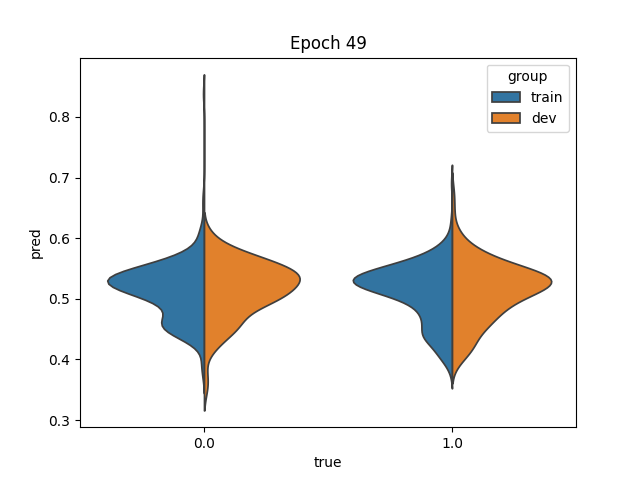
\includegraphics[width=3in]{img/3-1e49violin.png}}
    \caption{ABIDE CNN Model predictions at epoch 49 from \cite{aiad}.}
    \label{fig:xmp}
\end{figure}

\textbf{Even more figures are shown in Fig.~\ref{fig:xmp2}.} \lipsum[1]

\begin{figure}[htbp]
    \centerline{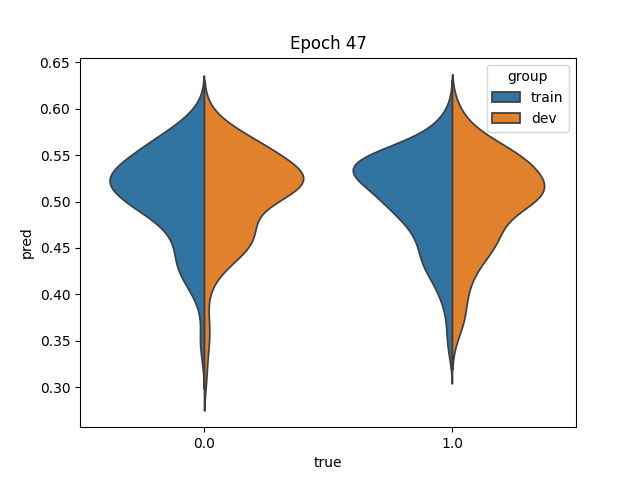
\includegraphics[width=3in]{img/3-1e47violin.png}}
    \centerline{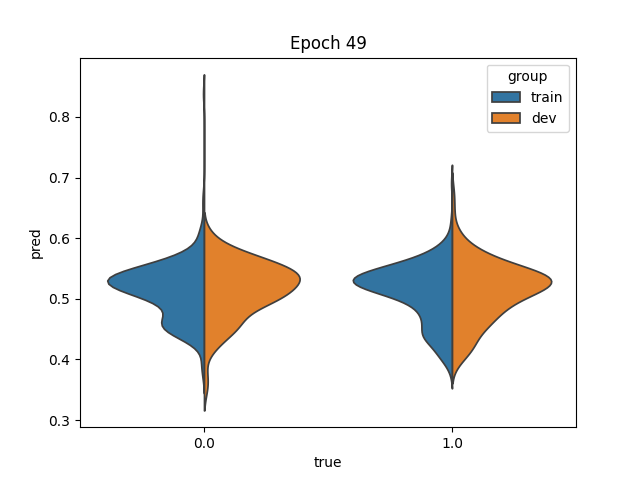
\includegraphics[width=3in]{img/3-1e49violin.png}}
    \caption{ABIDE CNN Model predictions at multiple epochs from \cite{aiad}.}
    \label{fig:xmp2}
\end{figure}

\textbf{An example of how to include a table is shown in Table~\ref{tab:xmp}.} \lipsum[1]

\begin{table}[htbp]
    \caption{Pointless table.}
    \begin{center}
        \begin{tabular}{|c|c|c|}
            \hline
            \textbf{C1} & \textbf{C2} & \textbf{C3} \\
            \hline
            1 & 2 & 3 \\
            4 & 5 & 6 \\
            7 & 8 & 9 \\
            \hline
        \end{tabular}
    \end{center}
    \label{tab:xmp}
\end{table}

\colorbox{red}{\color{white}{\textbf{NOTE: Positioning of the figs/tables known-bad -}}}
\colorbox{red}{\color{white}{\textbf{Will be refined when actual content is available.}}}

\lipsum[1-10]

\section{Conclusion} \label{CO}
\textbf{This is Trevor's Conclusion section.} \lipsum[1-2]

\section*{Acknowledgments}

Among others, we would like to thank Dr. Brian Hutchinson and Piper Wolters for their guidance and support throughout this project. \lipsum[][1-2]

\printbibliography
\end{document}
